\documentclass[acmsmall,nonacm,screen,review]{acmart}
\newif\ifEnableExtend
%\EnableExtendtrue
\EnableExtendfalse

\usepackage[utf8]{inputenc}
\usepackage{url}
\usepackage{color}
\newcommand{\csch}[1]{{\color{red} Christian says: #1}}
\newcommand{\Is}       {:=}
\newcommand{\set}[1]{\left\{ #1\right\}}
\newcommand{\sodass}{\,:\,}
\newcommand{\setGilt}[2]{\left\{ #1\sodass #2\right\}}
\usepackage{amsmath}
\usepackage{amsthm}
\usepackage{xspace}
\usepackage{relsize}
\usepackage{algorithm}
\usepackage{algpseudocode}
\usepackage{xcolor}
\usepackage{caption}
\usepackage{graphicx}
\usepackage{subcaption}
\usepackage{float}
\usepackage{numprint}




\newtheorem{openproblem}{Open Problem}
\newcommand{\ie}{i.\,e.,\xspace}
\newcommand{\eg}{e.\,g.,\xspace}
\newcommand{\etal}{et~al.\xspace}
\newcommand{\cov}{\term{cov}\xspace}
\newcommand{\term}[1]{\textsl{#1}}
%\newcommand{\Comment}[1]{\textsl{#1}}

%%%%%%%%%%%%%%%%%%%%%%%%%%%%%
\setcopyright{none}
\copyrightyear{2021}
\acmYear{2021}
\acmDOI{}
\acmPrice{}
\acmISBN{}

\title{Algorithm Engineering Practical: The Arc-Flags Algorithm}
\author{Marlon Dittes}
\email{hu256@stud.uni-heidelberg.de, BSc Informatik 100\%, 4164834}
\affiliation{%
  \institution{Heidelberg University}
  \streetaddress{Im Neuenheimer Feld 205}
  \city{Heidelberg}
  \state{Baden-Württemberg}
  \country{Germany}
  \postcode{69120}
}


\date{}

\begin{document}

\begin{abstract}
We look at how Dijkstra's Algorithm was modified to create the Arc-Flags Algorithm.
We clarify, which information the modified algorithm uses and how we can preprocess this information.
Furthermore, we run experiments on three different modifications of Dijkstra's Algorithm and compare query time, search space and speedup whilst looking at
different partitions.
\end{abstract}
\maketitle

\section{Introduction}
The shortest path problem is a fundamental graph theory question with multiple real-world applications. This problem plays a pivotal role in our daily lives,
particularly in applications such as GPS-based navigation systems for automobiles, where it enables us to efficiently find the quickest
routes to our destinations. Dijkstra's Algorithm~\cite{DBLP:books/mc/22/Dijkstra22a} has been the go-to tool for solving this problem, however, as networks grow larger and more complicated,
Dijkstra's Algorithm becomes less efficient.

In this report, we look at the speedup of Dijkstra's Algorithm by using Arc-Flags.
The Arc-Flags Algorithm, also known as the Arc-Flag Approach, is a goal-directed optimization technique for accelerating Dijkstra's Algorithm. The Arc-Flag
Approach, introduced by Möhring et al.~\cite{DBLP:journals/jea/MohringSSWW06},
attempts to reduce computation during Dijkstra's Algorithm by decreasing the amount of edges
that need to be considered, thus improving the efficiency.

The structure of this report is as follows: After first introducing the shortest path problem in Section~\ref{2} and Dijkstra's Algorithm, together
with its flaws, in Section~\ref{3},
we take a look at how the Arc-Flags Algorithm works and how we preprocess the information needed in Section~\ref{4}.
Furthermore, we show the results of various experiments in Section~\ref{5}.
Finally, we conclude in Section~\ref{6}.

\section{The shortest path problem}
\label{2}
A graph $G = (V,E)$ is a pair of nodes $V$ and directed edges $E$, where each edge $e_{u,v}$ is a pair of nodes $u,v \in V$.
Additionally, each edge is assigned a positive edge weight via a function $w \colon E \to \mathbb{R}^{+}$, $\quad w(e) = w_{e}$. For our purposes, this will
always just be the euclidean norm between the coordinates of the two nodes.

The shortest path problem then consists of finding a path $p = (v_1, v_2, \ldots, v_n)$, where $v_i \in V$ for $1 \leq i \leq n$, from the source node
$s = v_1 \in V$ to the target node $t = v_n \in V$, that minimizes the sum~$\sum_{i=1}^{n-1} w(e_{v_i, v_{i+1}})$.

This is called the \textit{single-pair shortest path problem}. Furthermore, we define the \textit{single-source shortest path problem},
in which we have to find the shortest paths from a source node $s$ to all other nodes in the graph, and the \textit{all-pairs shortest path problem},
in which we have to find shortest paths between every pair of nodes $u,v \in V$, which we will both be using later on.

\section{Dijkstra's Algorithm}
\label{3}
The go-to algorithm for solving the shortest path problem with non-negative edge weights is Dijkstra's Algorithm.
Dijkstra's Algorithm is a greedy algorithm that finds the shortest path between two nodes in a graph by iteratively selecting the node with the smallest known
distance and relaxing its adjacent edges.

\begin{algorithm}
  \captionsetup{labelformat=empty, labelsep=none}
  \caption{Dijkstra's Algorithm (G = (V, E), s, t)}
  \begin{algorithmic}[1]
      \State $dist[s] = 0$
      \State $Q.clear(), Q.add(s,0)$
      \While{$!Q.empty()$}
          \State $u \gets Q.deleteMin()$
          \For{all $edges$ e = (u,v) $\in E$}
              \If{$dist[u] + w_e < dist[v]$}
                  \State $dist[v] \gets dist[u] + w_e$
                  \If{$v \in Q$} \State $Q.decreaseKey(v, dist[v])$
                  \Else{} \State $Q.insert(v, dist[v])$
                  \EndIf
              \EndIf
          \EndFor
      \EndWhile
  \end{algorithmic}
\end{algorithm}

The algorithm uses a distance array $dist$, that saves the current shortest found distances for every node $n \in V$ from the source node $s$.
Additionally, we use a priority queue (binary heap) $Q$, to efficiently extract the closest unexplored node. In each iteration step the algorithm
extracts such a node $u \in V$ using $Q.deleteMin()$ and takes a look at all outgoing edges $e_{u,v}$, $v\in V$, from $u$ whilst analyzing, if the relaxation
criterion \colorbox{yellow}{$dist[u] + w_e < dist[v]$} is fulfilled. If this is the case, it either calls $Q.decreaseKey(v, dist[v])$ or
$Q.insert(v, dist[v])$, depending on if $v$ is already in $Q$ or not.

This variation of Dijkstra's Algorithm solves the \textit{single-source shortest path problem}, but we can easily modify it to solve the
\textit{single-pair shortest path problem} by adding an if statement after line 5, which checks if $v = t$ and exiting the while loop if true,
thus finishing Dijkstra's Algorithm early.

The main issue with Dijkstra's Algorithm is that it explores all nodes around the source node, essentially like an expanding circle. Dijkstra fails to put
more value on searching in the direction of the target node, which would make the algorithm explore fewer nodes, thus improving query time. Additionally, the
longer the path between the source and target, the more noticeable this phenomenon becomes, since for an increasing radius of this "circle", we explore
even more nodes that are unlikely for us to be necessary. 

\section{The Arc-Flags Algorithm}
\label{4}
This is where the Arc-Flags Algorithm by Möhring et al.~\cite{DBLP:journals/jea/MohringSSWW06} comes in.
The core idea of the algorithm involves partitioning the graph and then augmenting each edge with flag information during the preprocessing phase.
These flags are then used
to determine which edges should be analyzed further during the pathfinding process. The algorithm can be divided into three main steps: graph partitioning,
preprocessing flag information and pathfinding using the collected information.

\subsection{Algorithm}
\label{4.1}
We will first look at how we use the preprocessed information to improve query time.
To achieve the Arc-Flags Algorithm we just need to update the relaxation criterion of Dijkstra's Algorithm to be
\colorbox{yellow}{$dist[u] + w_e < dist[v]$ and $AF_{T}(e) = true$}, with $AF_{T}(e)$ being the Arc-Flag for the partition of the target~$t \in V$ (=:$T$) on the edge~$e \in E$.
Basically, we only need k flags for each edge $e$, where $k$ := number of blocks in a partition. This equates to an additional memory
consumption of $\Theta(k*|E|)$.

How it works is that, during pathfinding, each flag states, if the edge is part of any shortest path into the corresponding partition.
We can use this information to skip exploring edges, that we know are not going to be a part of the shortest path to $t$, reducing query time. As a matter of
course, we want to keep the percentage of set flags to a minimum.

\subsection{Preprocessing}
\label{4.2}
When it comes to the preprocessing step, there are two main problems we need to tackle. Firstly, we will need to partition the graph.
Secondly, we must consider how we actually compute the flag information that we use during the pathfinding.

\subsubsection{Partitioning}
For the partitioning, the graph partitioning program KaFFPa of KaHIP~\cite{DBLP:conf/wea/SandersS13} was used with preconfiguration set to strong. The speedup we get by using Arc-Flags is
heavily dependent on how good our partitions are, since, with bad partitions, we will hardly get any unset flags due to edges running into
various partitions. Hence, we need to use high quality partitions to maximize our possible speedup.

\subsubsection{Arc-Flag computation}
When it comes to computing the Arc-Flags, there are two approaches: naive and improved.
The naive approach consists of going through every node $n \in V$, inspecting which edges $e \in E$ are used for shortest paths leading into $n$ from all other
nodes and setting the corresponding flag of the partition of n(=:$N$) on all used edges. We do this by running backwards Dijkstra on every node $n \in V$,
which is the same as running Dijkstra from every node to $n$. We then extract the backwards shortest path tree and set the flag of $N$ to 1 for each tree
edge. By all means, this isn't very feasible, especially for larger graphs, since we get a running time of $O(m*n + n^2*log(n))$ for the
\textit{all-pairs shortest path problem} without negative edges.

The improved version aims to reduce the amount of times we need to run Dijkstra. Möhring et al.~\cite{DBLP:journals/jea/MohringSSWW06} show,
that it is sufficient to run backwards Dijkstra
on all so-called \textit{boundary nodes}. A boundary node $b \in V$  is defined as a node, where $\exists e_{b,v} \in E : partition(b) \neq partition(v)$.
They propose to once again extract the backwards shortest path tree from all boundary nodes $b$, using backwards Dijkstra, and set the corresponding Arc-Flag
to 1 for every tree edge. Additionally, for edges that run within a block $j$, we need to set the $j$-th flag.
This improved algorithm works due to the observation of all shortest paths not
running within a block passing through at least one boundary node.

\section{Experiments}
\label{5}
The experiments were implemented in C++ using partitions created by KaFFPa of KaHIP~\cite{DBLP:conf/wea/SandersS13} with preconfiguration set to strong.

In the following we will compare Dijkstra's Algorithm to three different variations: A-Star~\cite{DBLP:journals/sigart/HartNR72}, Arc-Flags and A-Star combined with Arc-Flags.
A-Star was chosen as a comparison due to it being an easy goal directed approach. This way, we can compare our Arc-Flags performance to another algorithm
that tries to improve Dijkstra in the same kind of way.

\subsubsection*{System}
All of our experiments were conducted on a server with an Intel(R) Xeon(R) CPU E5-2630 v2 @ 2.60GHz processor,
featuring \numprint{24} cores equipped with \numprint{62} GiB of RAM.
All programs were compiled with g++ 9.4.0 and the following flags: \texttt{-O3}.

\subsubsection*{Methodology}
For all experiments on the same dataset, the same \numprint{1000} random queries were used. Preprocessing was done in parallel, all other
experiments were done sequentially. For some graphics we used the arithmetic mean as an average over all \numprint{1000} random queries.

\subsubsection*{Datasets} 
Two datasets were used: Belgium and Germany. Belgium has \numprint{463514} nodes and \numprint{591882} undirected edges. Germany has \numprint{4378446}
nodes and \numprint{5483587} undirected edges.

\subsection{Preprocessing}

\begin{table}[bt!]
    \centering
    \caption{Overview of the results for the Belgium and Germany datasets depending on $k$, the number of blocks. The average query time is the arithmetic mean over all instances. Preprocessing was done in parallel on all 24 cores.
    $k=1$ shows Dijkstra's Algorithm, $k=1^*$ A-Star. The idea comes from~\cite{DBLP:conf/wea/GrossmannS0S23}.}
    \label{tab:experimental-results}
    \begin{subtable}{\textwidth} % First dataset: Belgium
        \caption{Belgium Dataset}
        \begin{tabular}{|c|c|c|c|c|c|}
            \hline
            $k$ & preproc. time & boundary nodes & avg. query time [ms] & memory [MB] & \% set flags \\
            \hline
            1 & - & - & 58.75 & - & - \\
            1* & - & - & 12.46 & - & - \\
            8 & 00:00:49 & 736 & 12.46 & 10.16 & 56.65\% \\
            16 & 00:01:57 & 1262 & 7.92 & 19.19 & 50.96\% \\
            32 & 00:03:16 & 2132 & 5.84 & 37.25 & 47.65\% \\
            64 & 00:04:23 & 3337 & 4.24 & 73.38 & 45.20\% \\
            128 & 00:05:18 & 5370 & 3.07 & 145.63 & 43.24\% \\
            256 & 00:13:15 & 8396 & 2.51 & 290.13 & 42.07\% \\
            512 & 00:19:58 & 13033 & 2.07 & 579.14 & 41.22\% \\
            \hline
        \end{tabular}
    \end{subtable}

    \vspace{10pt} % Add some vertical space between the two subtables

    \begin{subtable}{\textwidth} % Second dataset: Germany
        \caption{Germany Dataset}
        \begin{tabular}{|c|c|c|c|c|c|}
            \hline
            $k$ & preproc. time & boundary nodes & avg. query time [ms] & memory [MB] & \% set flags \\
            \hline
            1 & - & - & 703.87 & - & - \\
            1* & - & - & 175.33 & - & - \\
            8 & 00:13:52 & 1444 & 150.67 & 94.13 & 56.29\% \\
            16 & 00:37:36 & 2636 & 106.49 & 177.80 & 51.45\% \\
            32 & 01:11:01 & 4336 & 77.72 & 345.15 & 47.71\% \\
            64 & 02:00:33 & 6865 & 63.61 & 679.84 & 45.38\% \\
            128 & 03:01:25 & 10587 & 55.05 & 1349.23 & 43.75\% \\
            256 & 05:08:29 & 16935 & 48.88 & 2697.99 & 42.64\% \\
            \hline
        \end{tabular}
    \end{subtable}

    
\end{table}


In table~\ref{tab:experimental-results}, we realize that the preprocessing of the Arc-Flags information can become very costly, especially for the larger dataset (Germany).
This is the case, because on Germany we not only have way more boundary nodes for the same amount of blocks, but running backwards Dijkstra on every boundary
node also takes longer, because $|V|$ and $|E|$ are larger. 
When comparing the set flag percentages, we notice that we actually get the same kind of decrease for increasing block size on both datasets. 

\subsection{Comparison of algorithms}

\begin{figure}[bt!]
    \centering
    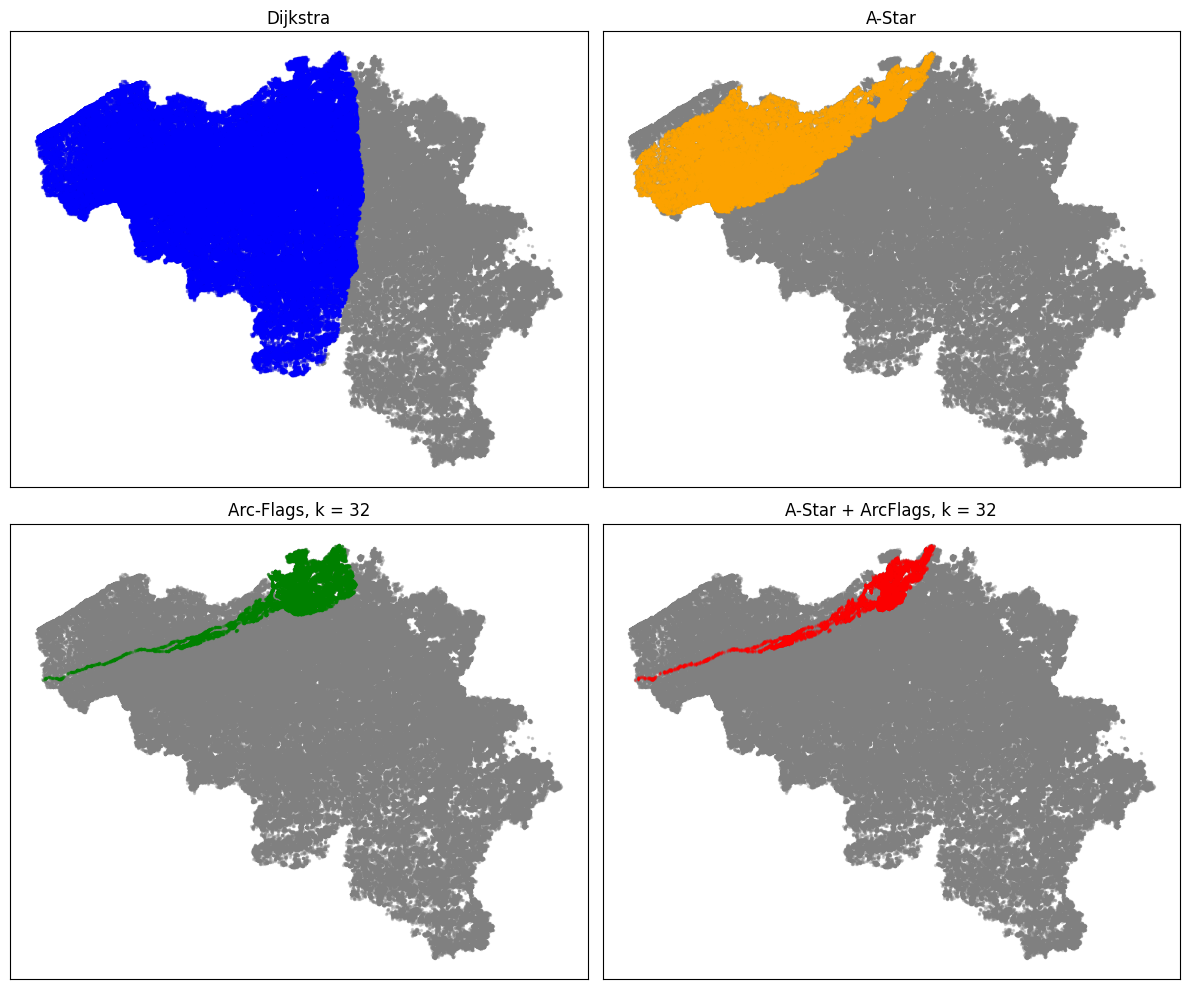
\includegraphics[width=0.6\linewidth]{subplots.png}
    \caption{Visualization of the four different algorithms on the Belgium dataset. The source node is on the left, the target node on the right.
    The gray points display the unexplored nodes, the colored points display the explored points of the corresponding algorithm.
    Number of partitions = 32.}
    \label{fig1}
\end{figure}

\begin{figure}[bt!]
    \centering
    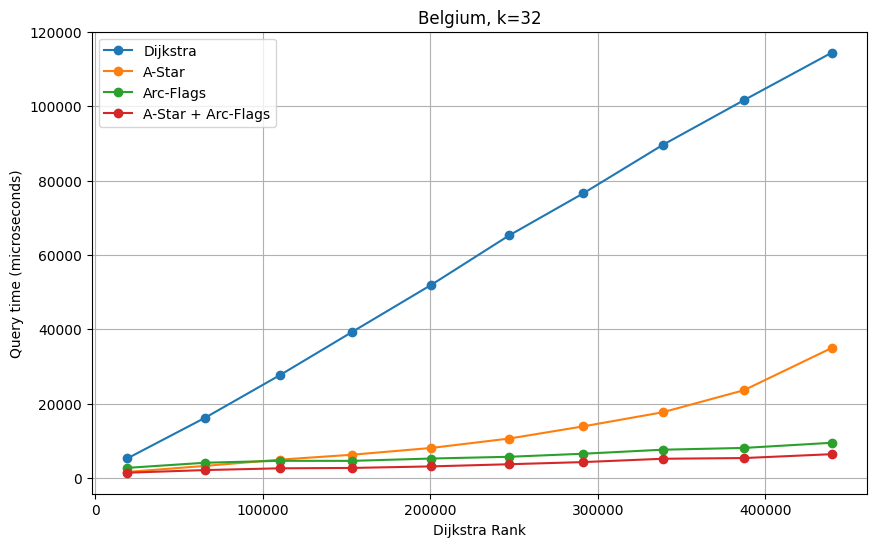
\includegraphics[width=0.6\linewidth]{belquery.png}
    \caption{Plots of the query times for the different algorithms on the Belgium dataset. The X-axis is Dijkstra Rank, the Y-axis is query time in microseconds.}
    \label{fig2}
\end{figure}

In this experiment we explore the different query times and search spaces of the four algorithms. 
In figure~\Ref{fig1} we notice the problem of Dijkstra searching in an expanding circle that we already mentioned earlier. We also notice that the A-Star Algorithm
significantly decreases the amount of nodes explored, but the Arc-Flags Algorithm with only \numprint{32} blocks is even better. It's important to mention the behavior
of the Arc-Flags Algorithm that we can see here: We initially explore few nodes when close to the source node, however, we need to explore way more nodes when
we're close to the target node. This is also where the biggest improvement of the A-Star + Arc-Flags combination comes in, which is just decreasing the
amount of nodes needed to explore close to the~target.

Figure \ref{fig2} then shows, that for smaller Dijkstra Rank, the A-Star Algorithm actually outperforms the Arc-Flag Algorithm. This is due to the fact
that for smaller Dijkstra Rank we are mostly searching a shortest path within a handful of partitions. Here we will
always be close to the target node, hence we have the mentioned problem of exploring more nodes. Additionally, if we only search within exactly one partition,
we also get no speedup from the Arc-Flag information because every flag is set to 1. Nonetheless, for bigger Dijkstra Rank, we notice that the Arc-Flags
Algorithm significantly outperforms the A-Star Algorithm, as illustrated in figure~\Ref{fig2}. Additionally, A-Star combined
with Arc-Flags always gives us a little better query times than simply Arc-Flags, mostly due to the target node phenomenon we noticed earlier.

\subsection{Comparison of partitions}

\begin{figure}[bt!]
    \centering
    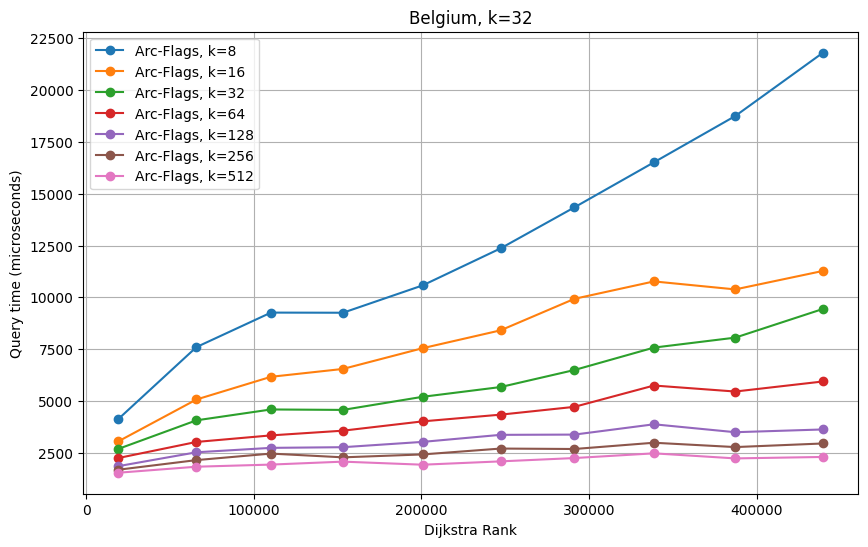
\includegraphics[width=0.49\linewidth]{arcflagDifferentKquery.png}
    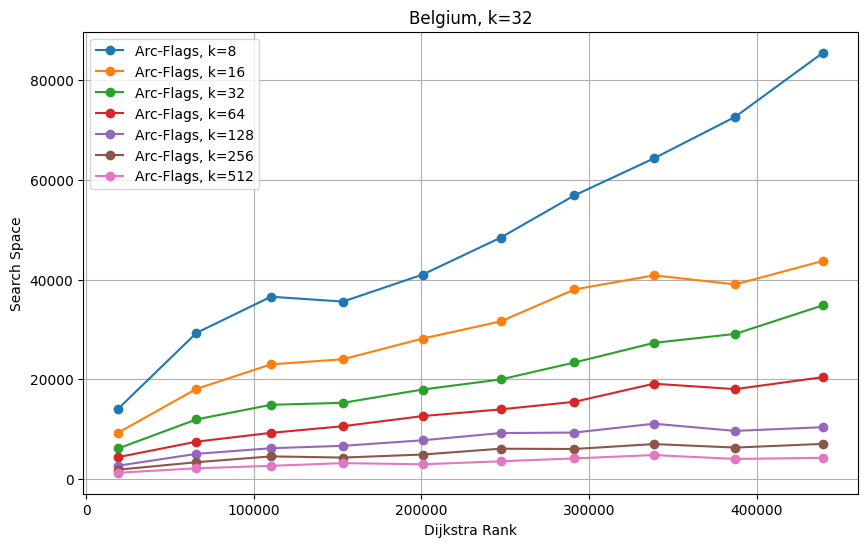
\includegraphics[width=0.49\linewidth]{arcflagDifferentKsearchspace.png}
    \caption{Comparison of the different query times and search spaces for the Arc-Flags Algorithm using different partitions on the Belgium dataset.
    The X-axis is Dijkstra Rank, the Y-axis is once query time in microseconds and once search space.}
    \label{fig3}
\end{figure}

\begin{figure}[bt!]
    \centering
    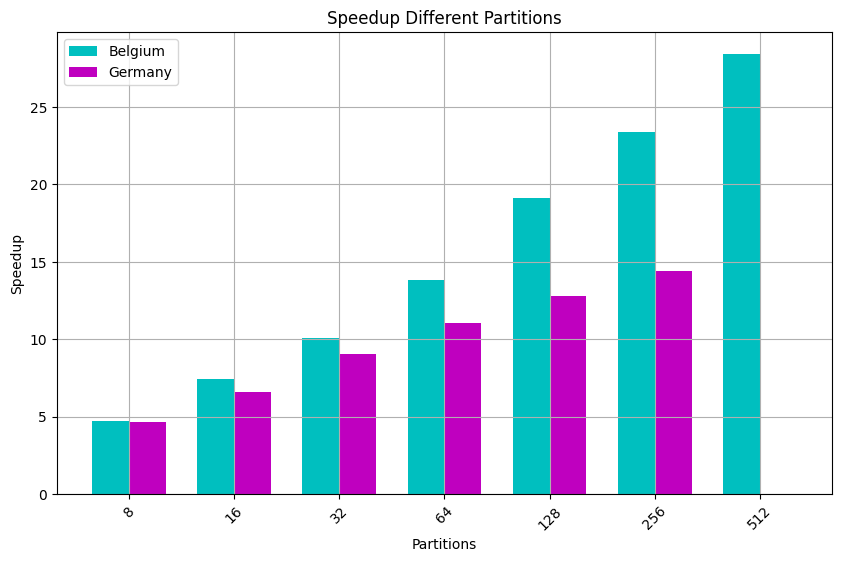
\includegraphics[width=0.6\linewidth]{combinedSpeedup.png}
    \caption{Speedup of Dijkstra's Algorithm by using Arc-Flags for different partitions on both datasets.
    On the X-axis are the different block counts of the partitions, on the Y-axis is the corresponding speedup.}
    \label{fig4}
\end{figure}

This experiment concerns the speedup for various partitions.
Figure~\ref{fig3} shows that the query times are mostly linear to the search space for all different partitions. This definitely makes sense, 
because the speedup we get by using Arc-Flags comes from exploring fewer nodes due to skipping certain edges. We can also see, that we always get a
speedup for the query time (or search space) when increasing the amount of blocks in a partition.
This is to be expected, because we have more flags per edge, thus more information to use during pathfinding.
It's important to mention that we always double the amount of blocks, however the improvement is way more significant for the first few sizes of $k$. Together
with the fact that it can take very long to preprocess the Arc-Flag information for bigger block counts (at least on bigger datasets like Germany), this makes
us want to use smaller $k$ sizes, because we have better cost-efficiency.

Figure~\Ref{fig4} shows us that we actually get better speedup for the Belgium dataset using the Arc-Flags Algorithm, at least for lower block counts.
This is mostly due to the memory consumption getting very big for the Germany dataset, as we can see in table~\Ref{tab:experimental-results}.
This makes it not very cache efficient, which slows down the pathfinding.
The speedup factors for the Belgium dataset are actually very good with up to about $28$ for k=512, especially because the preprocessing only
took around $20$ minutes (see table~\Ref{tab:experimental-results}). For Germany, we still have good speedup factors,
however the preprocessing took way longer than for Belgium.

\section{Conclusion}
\label{6}
In our experiments we showed that the Arc-Flag Approach is a feasible and powerful improvement for Dijkstra's Algorithm.
We have shown that it's very easy to modify Dijkstra to use Arc-Flag information. Additionally, we had a look at an easy way to compute the Arc-Flags in a
feasible manner. We also realize, that especially for lower block counts, we explore fewer nodes close to the source than we are exploring close to the target.

However, it is important to note that actually computing the information can become very expensive, especially for large graphs. Limitations of this approach
include its inability to deal with changing weights. 

Overall, we can conclude that the Arc-Flags Algorithm is a great goal-directed approach for improving Dijkstra's Algorithm, especially if the Arc-Flag
information is already provided. However, there is still some room left for improvement when it comes to preprocessing time, mainly for bigger graphs,
and certain exploring patterns.

\paragraph{Outlook}
Introducing a bidirectional Arc-Flag Approach could be very beneficial, since we observed that we explore fewer nodes close to the source and more
close to the target. If we were to use a bidirectional variant, we could make use of the narrow exploration from both sides until meeting somewhere
in the middle, without ever having to widen our exploration path. Since this phenomenon occurs particularly for lower block counts, we could settle for
Arc-Flags of partitions with fewer blocks, since most of the time save for more detailed partitions comes from finding the target node more efficiently.
By this argument, we would reduce our preprocessing computation time, one of the main problems that we encountered.

\bibliographystyle{plainnat}
\bibliography{references.bib}

\end{document}
